\begin{frame}[parent={ie:agenda}, hasnext=true, hasprev=false]
	\frametitle{ISO 15504}

	
	\begin{block:concept}{ISO 15504}
	\end{block:concept}
	
	\begin{block:fact}{Exemplos}
		\begin{itemize}
			\item Capacidade determinada pela avaliação dos processos executados pela
			empresa
		\end{itemize}
	\end{block:fact}
\end{frame}


\begin{frame}[hasnext=true, hasprev=true]
	\frametitle{ISO 15504}

	\begin{block:fact}{Níveis}
		\centering
		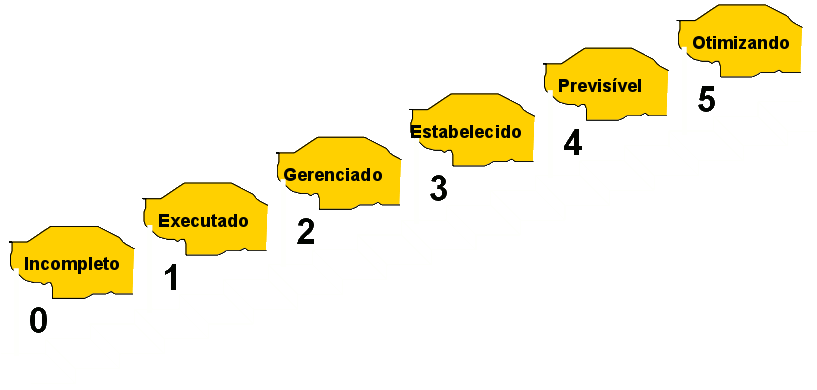
\includegraphics[width=\textwidth]{software-engineering/project-management/process/process-quality/iso15504/iso15504-steps}
	\end{block:fact}
\end{frame}

\begin{frame}
	\frametitle{ISO 15504}

	\begin{block:fact}{}
		Capacidade determinada pela avaliação dos processos executados pela empresa
	\end{block:fact}
	
	\begin{block:fact}{Atributos de processos (e níveis)}
		\begin{itemize}
			\item desempenho do processo (1)
			\item gerência do desempenho do processo (2)
			\item gerência do produtos de trabalho (2)
			\item definição de processo (3)
			\item instanciação de processo (3)
			\item medição de processo (4)
			\item controle de processo (4)
			\item inovação de processo (5)
			\item otimização de processo (5)
		\end{itemize}
	\end{block:fact}
\end{frame}

\begin{frame}[hasnext=false, hasprev=true]
	\frametitle{ISO 15504}

	\begin{block:fact}{Níveis}
		\centering
		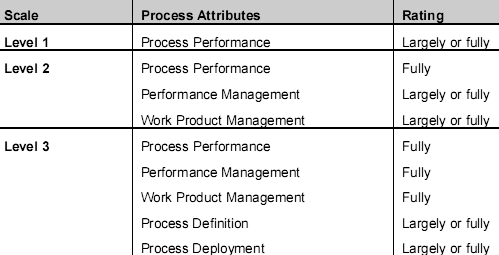
\includegraphics[width=\textwidth]{software-engineering/project-management/process/process-quality/iso15504/iso15504-rating-example}
	\end{block:fact}
\end{frame}

